\documentclass[12pt, a4paper, oneside]{ctexart}
\usepackage[margin=2cm]{geometry}%要先设置页边距,否则页眉页脚会偏
\usepackage{amsmath, amsthm, amssymb, bm, graphicx, hyperref, mathrsfs,float,xcolor,color}
\usepackage{listings}

% 用来设置附录中代码的样式

\lstset{
    basicstyle          =   \bf \ttfamily,          % 基本代码风格
    keywordstyle        =   \bfseries,   % 关键字风格
    keywordstyle        =   \color{blue},
    stringstyle         =   \color{magenta},
    commentstyle        =   \color{red}\ttfamily,
    language            =    [x86masm]Assembler,
    commentstyle        =   \rmfamily\itshape,  % 注释的风格,斜体
    escapeinside=``, % 英文分号中可写入中文
    stringstyle         =   \ttfamily,  % 字符串风格
    columns=fullflexible,%可以自动换行
    breaklines=true,%在单词边界处换行。
    numbers             =   left,   % 行号的位置在左边
    showspaces          =   false,  % 是否显示空格,显示了有点乱,所以不现实了
    numberstyle         =   \zihao{-5}\ttfamily,    % 行号的样式,小五号,tt等宽字体
    showstringspaces    =   false,
    captionpos          =   t,      % 这段代码的名字所呈现的位置,t指的是top上面
    frame               =   lrtb,   % 显示边框
}
\title{实验十 \qquad  键盘中断}
\author{学号:61822313 \qquad 姓名:钟锦程 \qquad 实验日期:\today}
\date{}
\begin{document}
\maketitle
\section{实验任务和实验结果}
\subsection{基础任务}
\subsubsection{实验任务的具体内容}
要求每按下任意一个键就向CPU发出中断请求信号,该信号由8259的IRQ1引入,中断类型号为09,CPU响应中断后转入执行KEYINTS中断服务程序,并在屏幕上显示“OK!”,按下10次键后返回DOS。
\subsubsection{调试通过的源程序}
\begin{lstlisting}
DATA SEGMENT
    OKSTR DB 'OK!',0DH,0AH,'$'
    TIME DB 00H
    NINE EQU 9
DATA ENDS;TIME是按键次数
STACK  SEGMENT
	DW 200H DUP(?)
STACK ENDS
CODE SEGMENT 
    ASSUME CS:CODE,DS:DATA,SS:STACK
DELAY PROC         ; 延时程序
    PUSH CX
    PUSH DX
    MOV DX,36H
DL500:
    MOV CX, 08FFFH
DL10MS:
    LOOP DL10MS
    DEC DX
    JNZ DL500
    POP DX
    POP CX    
    RET
DELAY ENDP

DELAY2 PROC         ; 延时程序2,用于显示OK时的延时,略短于1秒
    PUSH CX
    PUSH DX
    MOV DX,16H
DL5002:
    MOV CX, 01FFFH
DL10MS2:
    LOOP DL10MS2
    DEC DX
    JNZ DL5002
    POP DX
    POP CX    
    RET
DELAY2 ENDP
DISP1 PROC FAR     ; 显示太阳
    PUSH AX
    PUSH BX
    PUSH CX
    PUSH DX
    MOV AH,15     ; 读当前显示状态
    INT 10H
    MOV AH,0      ; 设置显示方式
    INT 10H
    MOV DX,0      ; 行号为0,列号为0
REPT: 
    MOV AH,2      ; 设置光标位置
    INT 10H  
    MOV AL,0FH    ; OFH是太阳图形的ASCII码
    MOV CX,1      ; 重复字符的次数
    MOV AH,10     ; 写字符
    INT 10H
    CALL DELAY
    SUB AL,AL
    MOV AH,0      ; 清除原图形
    INT 10H
    INC DH        ; 行号+1
    ADD DL,2      ; 列号+2
    CMP DH,20     ; 判断是否到20行,不等继续显示太阳,相等返回,如果到25行再返回,会导致轨迹不是严格对角
    JNE REPT
    POP DX
    POP CX
    POP BX
    POP AX
    RET
DISP1 ENDP
DISP2 PROC FAR    ; 显示OK
    PUSH CX
    PUSH BX
    PUSH AX
    MOV CX,3;待显示的字符数
NEXTC: 
    LODSB  ; 字符串"OK!"在数据段中定义,AL<—[SI]
    MOV AH, 0EH ; 用teletype格式写字符,并移动光标
    MOV BX,1
    INT 10H
    CALL DELAY2
    LOOP NEXTC
    POP AX
    POP BX
    POP CX
    RET
DISP2 ENDP

KEYINT PROC FAR 
    PUSH AX
    PUSH BX 
    PUSH DX 
    STI 
    IN AL,60H      ; 通过8255A的PA口(PA口地址为60H)读取键盘扫描码
    MOV AH,AL
    IN AL,61H      ; 从8255APB口(PB口地址为61H)的PB7输出一个正脉冲
    OR AL,80H      ; PB7置1
    OUT 61H,AL
    AND AL,7FH      ; PB7清零
    OUT 61H,AL     ;再输出一个负脉冲
    TEST AH,80H    ; 相等时代表键被释放,开中断,显示字符
    JNE BACK         ; 不等,中断结束返回
    STI  
    INC TIME 
    MOV SI,OFFSET OKSTR   ; 初始化SI,在DISP2中不再对SI进行初始化
    CALL DISP2
BACK:
    MOV AL,20H
    OUT 20H,AL
    POP DX
    POP BX
    POP AX
    IRET 
    KEYINT ENDP 
START:
    MOV AX,DATA 
    MOV DS,AX 
    MOV AX,STACK
    MOV SS,AX
    MOV AX,0
    MOV ES,AX
    MOV SI,OFFSET OKSTR
    MOV AX,ES:[24H]   ; 9*4=24H,压入中断向量的偏移地址
    PUSH AX
    MOV AX,ES:[26H]   ;压入中断向量的段地址
    PUSH AX
    CLI;关中断,载入自定义中断子程序地址时不允许中断
    MOV AX,SEG KEYINT 
    MOV ES:[26H],AX 
    MOV AX,OFFSET KEYINT
    MOV ES:[24H],AX
    STI
AGIN:
    CALL DISP1
    CMP TIME,10
    JB AGIN 
    CLI               ; 禁止下方程序中断发生,保护代码运行
    POP AX
    MOV ES:[26H],AX;弹出原中断向量的段地址
    POP AX
    MOV ES:[24H],AX;弹出原中断向量的偏移地址
    STI               ; 开中断
    MOV AH,4CH
    INT 21H
CODE ENDS
END START 


\end{lstlisting}
\subsubsection{实验结果}
如图\ref{基础实验结果截图1}是程序正常运行的截图,如果不按键,则当图标走到右下角后会从左上角重新开始,循环往复。图\ref{基础实验结果截图2}是按一次键的运行截图。可以看到在本应显示太阳符号的地方显示"OK!",如果多次按键(或长按),会不间断显示"OK!"(如图\ref{基础实验结果截图3}),直到所有"OK!"显示完毕才会继续显示太阳符号。当按键总次数达到10次时,程序会在本次太阳显示循环结束后中止程序,如图\ref{基础实验结果截图4}。
\begin{figure}[H]
    \centering
    \begin{minipage}{0.45\textwidth}
    \centering
    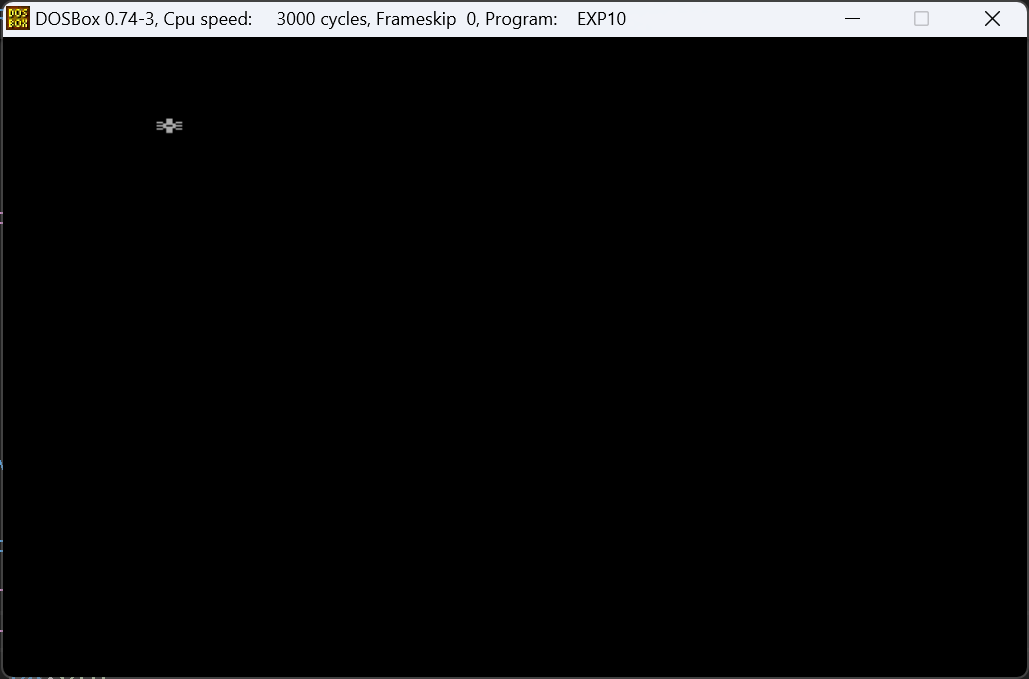
\includegraphics[scale=0.48]{pic/exp10-1.png}
    \caption{基础实验任务结果截图1}
    \label{基础实验结果截图1}
    \end{minipage}
    \hspace{0.05\textwidth}
    \begin{minipage}{0.45\textwidth}
    \centering
    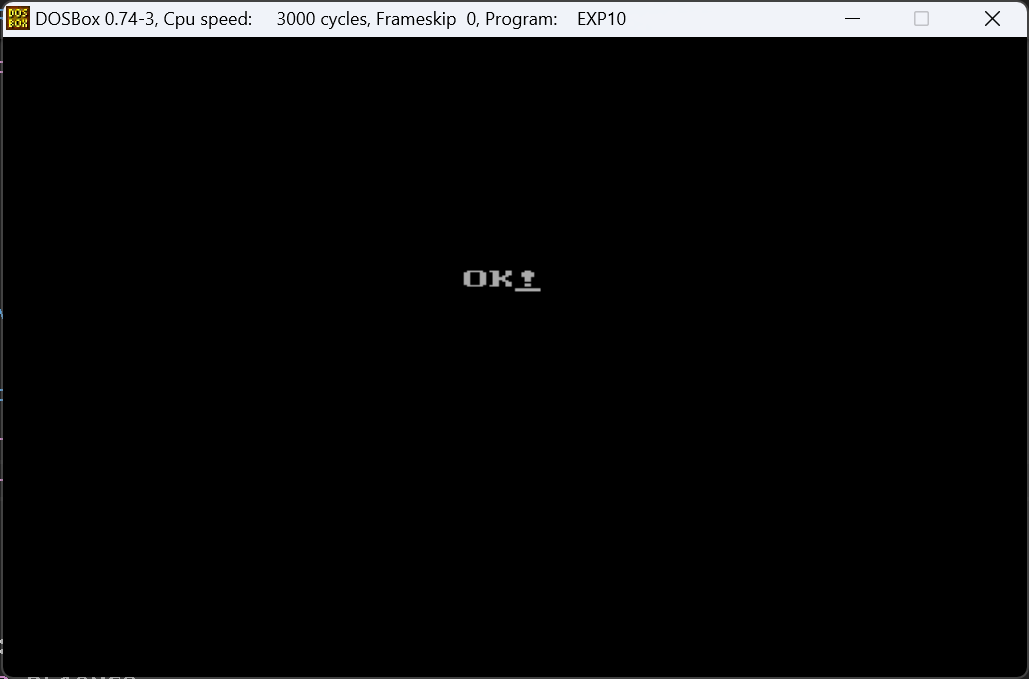
\includegraphics[scale=0.48]{pic/exp10-2.png}
    \caption{基础实验任务结果截图2}
    \label{基础实验结果截图2}
    \end{minipage}
\end{figure}
\begin{figure}[H]
    \centering
    \begin{minipage}{0.45\textwidth}
    \centering
    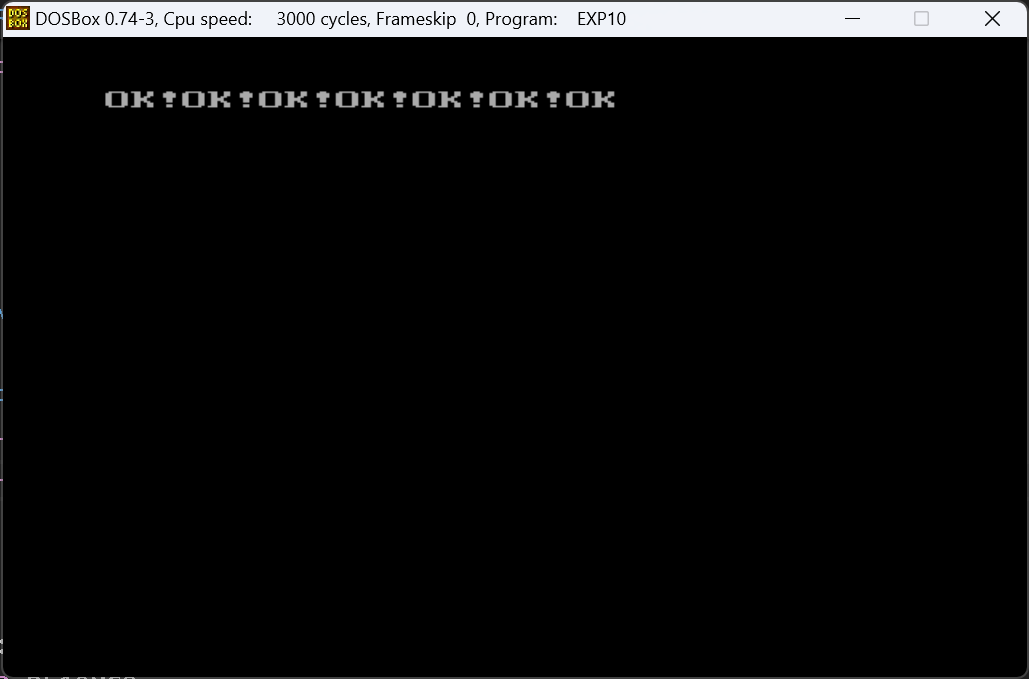
\includegraphics[scale=0.48]{pic/exp10-3.png}
    \caption{基础实验任务结果截图1}
    \label{基础实验结果截图3}
    \end{minipage}
    \hspace{0.05\textwidth}
    \begin{minipage}{0.45\textwidth}
    \centering
    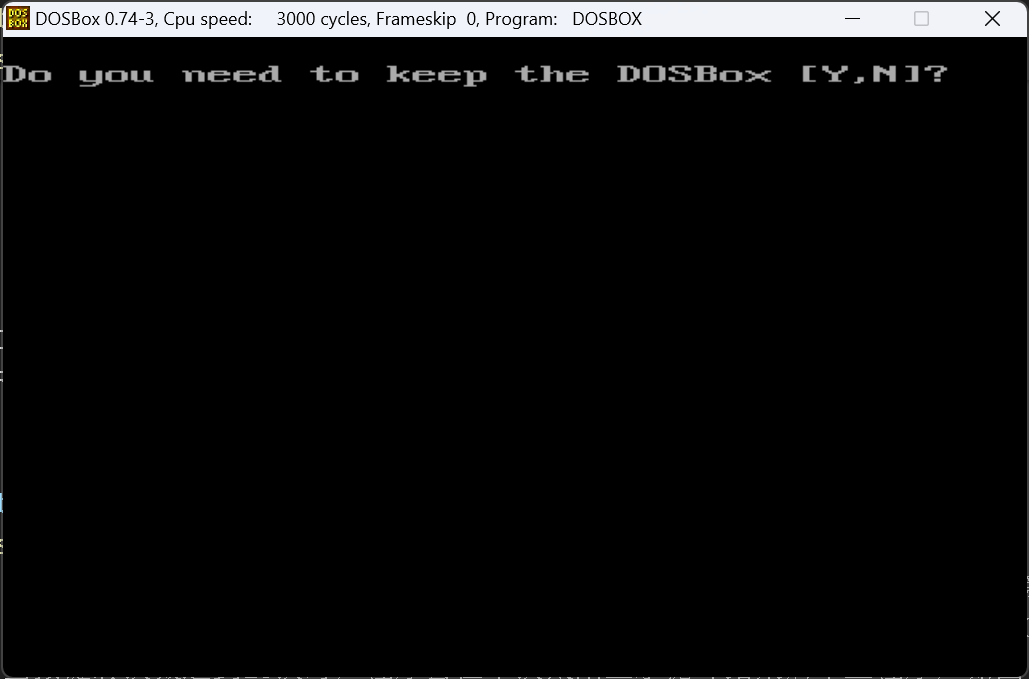
\includegraphics[scale=0.48]{pic/exp10-4.png}
    \caption{基础实验任务结果截图2}
    \label{基础实验结果截图4}
    \end{minipage}
\end{figure}
\subsection{附加任务}
\subsubsection{实验任务的具体内容}
1)通过DOS系统功能调用的25H、35H功能实现中断向量的设置和读取;

2)改变按键后屏幕显示的字符串内容和返回DOS之前的按键次数,比如:按键后在屏幕上显示“KEYINT”,按下9次键后返回DOS.按键显示的字符串内容和返回DOS之前的按键次数 各位同学可以自己设置,尽量不要太雷同,要求显示字符串的字符个数>3,按键次数>8。

3)在按键后显示的字符串前面加上按键次数,在字符串后面加个空格,这样两次按键显示字符串之间有个空格间隔区分一下;

4)按键次数达到后(比如9次),不等25行太阳图标显示完,立即返回DOS;

5)修改显示字符的属性,如,红底白字,蓝底黄字
\subsubsection{调试通过的源程序}
\begin{lstlisting}
DATA SEGMENT
    TIME DB 00H
    SHOWTIME DB 00H;SHOWTIME存放TIME对应的ASCII码
    OKSTR DB 'HI,ZJC!',20H
    N EQU $-SHOWTIME
    COUNT DB N;COUNT用于在显示过程中计数递减,便于直接中断而不用等本次太阳循环结束
    NINE EQU 9;定义数值常量便于调试
DATA ENDS;TIME是按键次数
STACK  SEGMENT
	DW 200H DUP(?)
STACK ENDS
CODE SEGMENT 
    ASSUME CS:CODE,DS:DATA,SS:STACK
DELAY PROC         ; 延时程序
    PUSH CX
    PUSH DX
    MOV DX,36H
DL500:
    MOV CX, 08FFFH
DL10MS:
    LOOP DL10MS
    DEC DX
    JNZ DL500
    POP DX
    POP CX    
    RET
DELAY ENDP

DELAY2 PROC         ; 延时程序2
    PUSH CX
    PUSH DX
    MOV DX,16H
DL5002:
    MOV CX, 01FFFH
DL10MS2:
    LOOP DL10MS2
    DEC DX
    JNZ DL5002
    POP DX
    POP CX    
    RET
DELAY2 ENDP

DISP1 PROC FAR     ; 显示太阳
    PUSH AX
    PUSH BX
    PUSH CX
    PUSH DX
    MOV AH,15     ; 读当前显示状态
    INT 10H
    MOV AL,1
    MOV AH,0      ; 设置显示方式
    INT 10H
    MOV DX,0      ; 行号为0,列号为0
REPT: 
    MOV AH,2      ; 设置光标位置
    INT 10H  
    MOV AL,0FH    ; OFH是太阳图形的ASCII码
    MOV CX,1      ; 重复字符的次数
    MOV BL,14H    ;字符颜色信息为白底红字加闪烁(b7控制字符是否闪烁,b6-b4为背景色,b3-b0为前景色)
    MOV AH,9     ; 写字符
    INT 10H
    CALL DELAY
    SUB AL,AL
    MOV AH,0      ; 清除原图形
    INT 10H
    CMP TIME,NINE;当次数达到设定值时,直接结束显示
    JAE QUIT1 
    INC DH        ; 行号+1
    ADD DL,2      ; 列号+2
    CMP DH,20     ; 判断是否到20行,不等则继续显示太阳,相等返回
    JNE REPT
QUIT1:
    POP DX
    POP CX
    POP BX
    POP AX
    RET
DISP1 ENDP

DISP2 PROC FAR    ; 中断显示信息
; INT 10H 中AH=03H读取光标信息。入口参数:BH=显示页码
; 出口参数:CH=光标的起始行 CL=光标的终止行 DH=行(Y坐标) DL=列 (X坐标)
    PUSH DX
    PUSH CX
    PUSH BX
    PUSH AX
    MOV COUNT,N;用待显示的字符串的长度更新COUNT
NEXTC: 
    LODSB  ; 字符串在数据段中定义并已经由SI指向首址
    MOV BH,00H
    MOV AH,03H
    INT 10H 
    MOV AH,9   ;写字符
    MOV CX,1      ;重复一次
    MOV BL,24H    ;字符颜色信息为绿底红字
    INT 10H
    INC DL ;每打印1个字符,光标的列号+1
    MOV AH,2      ; 更新光标位置
    INT 10H 
    CALL DELAY2 
    DEC COUNT  
    CMP COUNT,0 ;当整个中断信息串都显示完,才退出循环
    JA NEXTC
    POP AX
    POP BX
    POP CX
    POP DX
    RET
DISP2 ENDP

KEYINT PROC FAR 
    PUSH AX
    PUSH BX 
    PUSH DX 
    STI 
    IN AL,60H      ; 通过8255A的PA口(PA口地址为60H)读取键盘扫描码
    MOV AH,AL
    IN AL,61H      ; 从8255APB口(PB口地址为61H)的PB7输出一个正脉冲(即PB7先输出高电平,再输出低电平)
    OR AL,80H      ; PB7置1
    OUT 61H,AL
    AND AL,7FH; PB7清零
    OUT 61H,AL     
    TEST AH,80H    ; 相等时代表键被释放,开中断,显示字符
    JNE BACK         
    STI  
    INC TIME 
    MOV AL,0
    ADD AL,TIME 
    OR AL,30H
    MOV SI,OFFSET SHOWTIME   ; 初始化SI,使其指向中断信息字符串首址
    MOV [SI],AL
    CALL DISP2
BACK:
    MOV AL,20H
    OUT 20H,AL;结束中断
    POP DX
    POP BX
    POP AX
    IRET 
    KEYINT ENDP 

START:
    MOV AX,DATA 
    MOV DS,AX 
    MOV AX,STACK
    MOV SS,AX
    MOV AX,0
    MOV ES,AX
    MOV SI,OFFSET TIME
    MOV AH,35H ;INT 21H 35H号:取中断向量,入口AL=中断类型,出口ES:BX=中断向量
    MOV AL,9
    INT 21H 
    PUSH BX ;将原中断处理程序的CS:IP压栈
    PUSH ES 
    MOV AX,0 ;恢复ES!重要!
    MOV ES,AX
    PUSH DS ;保护DS与DX!重要!
    PUSH DX
    CLI
    MOV AX,SEG KEYINT ;将自定义中断服务程序的地址放入原09号中断向量处
    MOV DS,AX
    MOV DX,OFFSET KEYINT
    MOV AL,9
    MOV AH,25H ;INT 21H 25H号:设置中断向量,入口DS:DX=中断向量,AL=中断类型号
    INT 21H
    STI
    POP DX 
    POP DS 
AGIN:
    CALL DISP1
    CMP TIME,NINE
    JB AGIN 
    CLI               ; 禁止下方程序中断发生,保护代码运行
    POP DS  ;恢复原09号中断向量
    POP DX
    MOV AL,9
    MOV AH,25H
    INT 21H
    STI               ; 开中断
    MOV AH,4CH
    INT 21H
CODE ENDS
END START 


\end{lstlisting}
\subsubsection{实验结果}
如图\ref{附加实验任务结果截图1}是程序正常运行的截图,太阳符号被修改为白底红字加闪烁(附加功能5、6)。图\ref{附加实验任务结果截图2}是按一次键的运行截图。显示了绿底红字的中断信息"HI!ZJC"并在该字符串前面显示了按键次数(附加功能2)。图\ref{附加实验任务结果截图3}是长时间按键的截图,程序不断打印中断信息,信息之间有空格(附加功能3)。图\ref{附加实验任务结果截图4}是按键次数达到9次时的截图,可以看到程序直接退出返回DOS,而非等到本次太阳显示完才结束(附加功能4)。(附加功能1可从程序源代码中看到)
\begin{figure}[H]
    \centering
    \begin{minipage}{0.45\textwidth}
    \centering
    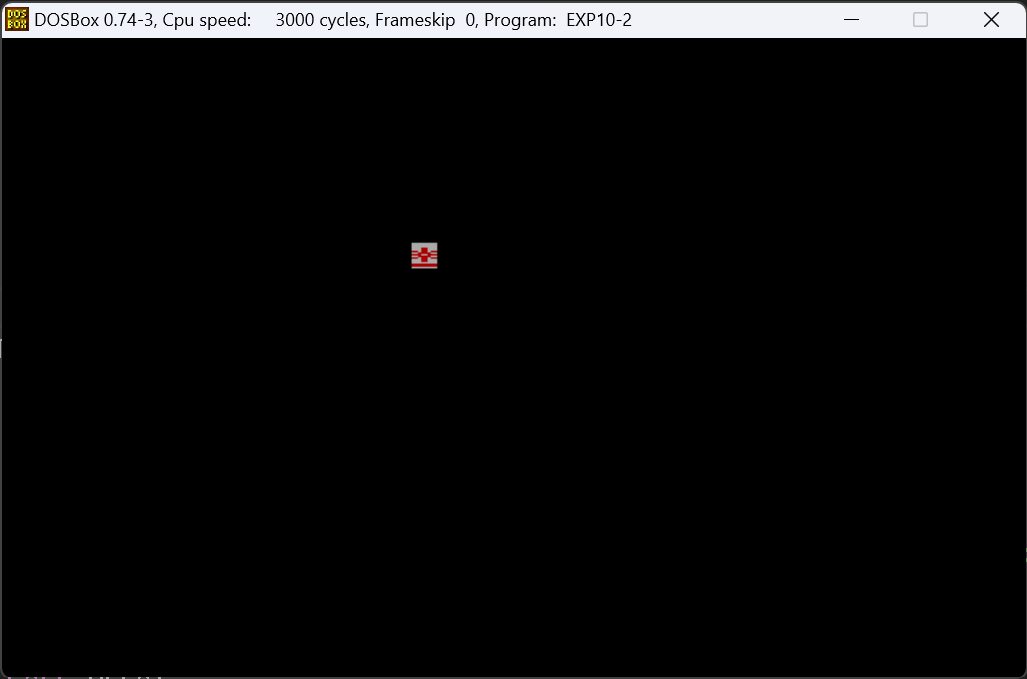
\includegraphics[scale=0.48]{pic/exp10-5.png}
    \caption{附加实验任务结果截图1}
    \label{附加实验任务结果截图1}
    \end{minipage}
    \hspace{0.05\textwidth}
    \begin{minipage}{0.45\textwidth}
    \centering
    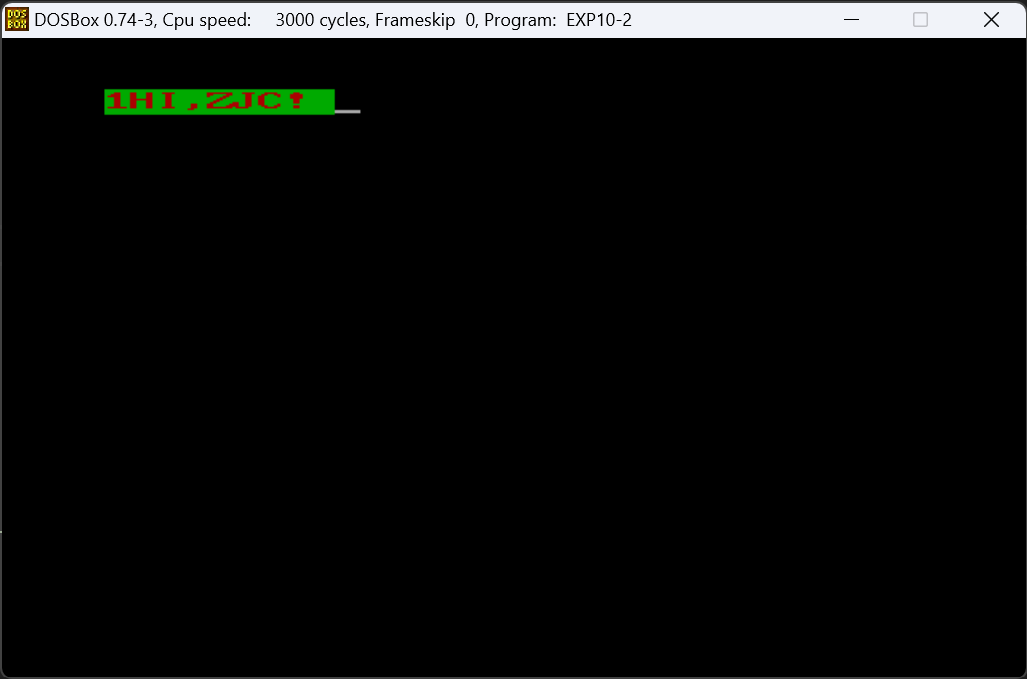
\includegraphics[scale=0.48]{pic/exp10-6.png}
    \caption{附加实验任务结果截图2}
    \label{附加实验任务结果截图2}
    \end{minipage}
\end{figure}
\begin{figure}[H]
    \centering
    \begin{minipage}{0.45\textwidth}
    \centering
    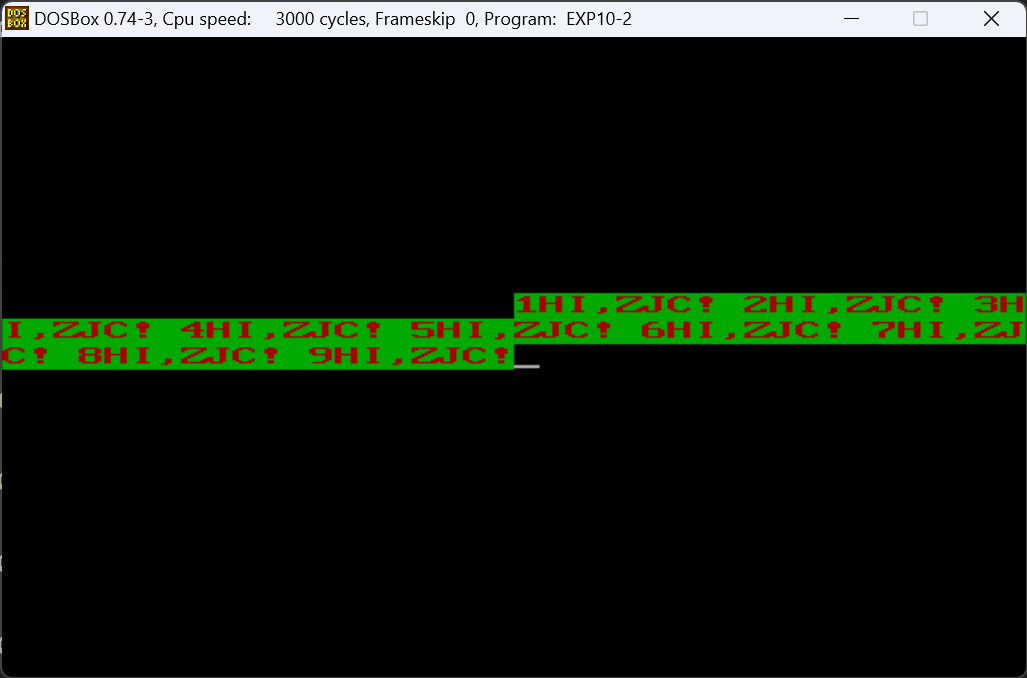
\includegraphics[scale=0.48]{pic/exp10-7.png}
    \caption{附加实验任务结果截图3}
    \label{附加实验任务结果截图3}
    \end{minipage}
    \hspace{0.05\textwidth}
    \begin{minipage}{0.45\textwidth}
    \centering
    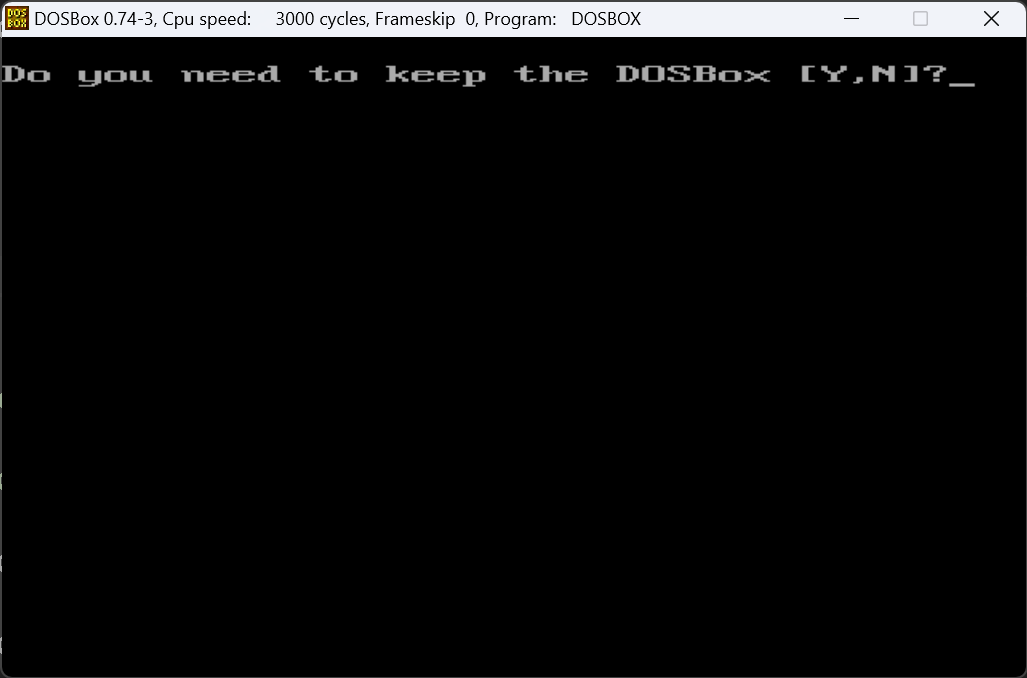
\includegraphics[scale=0.48]{pic/exp10-8.png}
    \caption{附加实验任务结果截图4}
    \label{附加实验任务结果截图4}
    \end{minipage}
\end{figure}
\section{实验总结}
本次实验首次接触键盘中断,对自定义中断服务程序的流程不熟悉,并且还没有形成保护现场的习惯。在用DOS中断服务(AH=25H INT 21H)编写中断服务程序KEYINT时,由于没有保护ES的值,导致读取中断向量后ES被改变,中断程序跳转错误。在输入键扫描码,键状态触发器复位的设计过程中也遇到了不小的困难。

另外,在本次实验中较为细致的学习了屏幕显示的相关知识,比如设置显示参数,控制光标等等。编写程序时比较麻烦的一点就是对光标的控制。如果要自定义字符属性就不能使用Teletype方法打印,而必须自己手动控制光标位置。
\section{思考题}
% 1. 键盘上某个键按下和释放时都会向8259发出中断请求,要求只在键按下时显示'OK!',键释放时不显示,在中断服务程序KEYINTS中是如何实现的?
% 2. 完成附加功能4(按键次数达到后(比如9次),不等25行太阳图标显示完,立即返回DOS)的同学,请简要说明:
% 1)是如何实现该附加功能的?
% 2)如果程序运行结束后,键盘不能正常使用(按键没反应),可能是哪些原因?

\begin{enumerate}
    \item 当键盘上的一个按键按下时,键盘会发送一个中断信号给CPU,与此同时,键盘会在指定端口(0x60) 输出一个数值a,当按键弹起时,键盘又给端口输出一个数值b.通过查表得,a的最高位都是0,b的最高位都是1,因此若按键释放,指令TEST AH,80H使ZF=1,后续JNE指令跳转到BACK,直接退出KEYINT,不显示字符。
    \item 附加功能如何实现:修改DISP1子程序,在REPT部分加入指令CMP TIME,NINE和JAE QUIT1,当按键达到指定次数时直接跳转到退出部分,而不需等待本次显示结束。
    \item 键盘不能正常使用的可能原因:在程序末尾没有恢复原09号中断向量的内容,导致键盘中断处理异常。
\end{enumerate}


\end{document}